\section{Feature-First Block Model}

In this section we propose a novel generative model for labelled networks. We call this the feature-first block model (FFBM -- illustrated in Figure~\ref{fig:ffbm}).

Let $N$ denote the number of vertices, $B$ the number of blocks
and ${\cal X}$ the set of values each feature can take.
We define the vector $x_i \in \Xcal^D$ as the feature vector for vertex $i$, 
where $D$ is the number of features associated with each vertex.
For the datasets we analyse, we deal with binary feature flags so $\Xcal = \{0, 1\}$. We write $X$ for the $N\times D$ {\em feature matrix} containing
the feature vectors $\{x_i\}_{i=1}^{N}$ 
as its rows.

For the FFBM, we start with the feature matrix $X$ and generate a random
vector of block memberships $b \in [B]^N$. For each vertex $i$, the
block membership $b_i\in[B]$ is generated based on the feature
vector $x_i$, independently between vertices. The conditional
distribution of $b_i$ given $x_i$ also depends on a collection
of weight vectors $\theta=\{w_k\}_{k=1}^B$, where each
$w_k$ has dimension $D$. We will later find it convenient
to write $\theta$ as a $B \times D$ matrix of weights $W$. Specifically, 
the distribution of $b$ given $X$ and $\theta$ is,
%
\begin{equation}
	p(b| X, \theta) = \prod_{i \in [N]} p(b_i | x_i, \theta) = \prod_{i \in [N]} \phi_{b_i} (x_i; \theta)
	= \prod_{i \in [N]} \frac{\exp\left(w_{b_i}^T x_i\right)}{\sum_{k \in [B]} \exp \left( w_k^T x_i\right)}.
\end{equation}

Note that $\phi_{b_i}$ has the form of a softmax activation function.
More complex models based on different choices for the distributions
$\phi_{b_i}$ above are also possible, but then deriving meaning from 
the inferred parameter distributions is more difficult. 
%
\begin{figure}
	\centering
	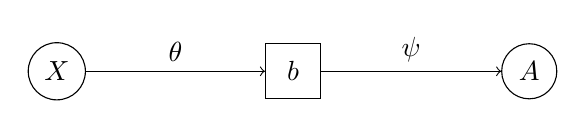
\begin{tikzpicture}[
		roundnode/.style={circle, draw=black, minimum size=7mm},
		squarednode/.style={rectangle, draw=black, minimum size=7mm}
		]
		% nodes
		\node[roundnode] (X) at (0, 0) {$X$};
		\node[squarednode] (b) at (3, 0) {$b$};
		\node[roundnode] (A) at (6, 0) {$A$};
		
		% arrows
		\draw[->] (X.east) -- node[above] {$\theta$} (b.west);
		\draw[->] (b.east) -- node[above] {$\psi$}(A.west);
	\end{tikzpicture}
	\caption{The Feature-First Block Model (FFBM)}
	\label{fig:ffbm}
\end{figure}

Once the block memberships $b$ have been generated, we then draw the 
graph $A$ from the microcanonical DC-SBM with additional parameters 
$\psi = \{\psi_e, \psi_k\}$:
%
\begin{equation}
	A \sim \textrm{DC-SBM}_{\textrm{MC}} (b, \psi_e, \psi_k).
	\label{eqn:A-generation}
\end{equation}

\subsection{Prior selection}

To complete the description of our Bayesian framework,
priors on $\theta$ and $\psi$ must also be specified. 
We place a Gaussian prior on $\theta$ such that
each element of $\theta$ has an independent ${\cal N}(0,\sigma_\theta^2)$
prior, with hyperparameter $\sigma_\theta^2$:
%
\begin{equation}
	p(\theta) \sim \Gaussian \left( \theta ; 0, \sigma_\theta^2 I \right).
	\label{eqn:theta-prior}
\end{equation}

This choice of prior gives a very
simple form for the conditional distribution of the block membership vector $b$ given $X$; it is a uniform distribution:
%
\begin{equation}
	p(b | X) = \int p(b | X, \theta) p(\theta) d\theta = B^{-N}.
	\label{eqn:b-pseudo-prior}
\end{equation}

The proof is given in Appendix~\ref{appdx:b|x}. This an important simplification as evaluating $p(b | X)$ does not require an expensive  integration over $\theta$ nor does it require the exact value of $X$.
Peixoto \cite{Peixoto-Bayesian-Microcanonical} proposes careful choices for 
the priors on the additional microcanonical SBM parameters $\psi$, which we adopt. 
The idea is to write the joint distribution on $(b, e, k)$ as a product of 
conditionals, $p(b, e, k) = p(b) p(e | b) p(k | e, b)= p(b) p(\psi | b)$. 
In our case, conditioning on $X$ is also necessary, leading to,
$
	p(b, \psi | X) = p(b | X) p(\psi | b, X) = p(b | X) p(\psi | b),
$
where we used the fact $\psi$ and $X$ are conditionally 
independent given $b$.
All that concerns the main argument is that it has
an easily computable form.
